\documentclass[12pt]{book} 
\usepackage{fullpage} 
\usepackage{graphicx} 
\usepackage[utf8]{inputenc}
\usepackage[italian]{babel}
\usepackage{setspace}
\usepackage{color}
\usepackage{xcolor}
\usepackage{listings}

\usepackage{caption}
\DeclareCaptionFont{white}{\color{white}}
\DeclareCaptionFormat{listing}{\colorbox{gray}{\parbox{\textwidth}{#1#2#3}}}
\captionsetup[lstlisting]{format=listing,labelfont=white,textfont=white}

\title{Sviluppo della gestione delle note di credito in un programma di fatturazione}
\author{Davide Fontana}
\begin{document}
\maketitle
\tableofcontents
\chapter{Introduzione}
%Introduzione
Questa relazione riguarda il tirocinio da me effettuato presso l' azienda 
Consoft Informatica S.r.l tra Febbraio e Aprile 2016 nella sede di Padova.
Lo stage è cominciato con una prima parte di formazione sulle tecnologie usate 
all'interno dell'azienda tra cui Java J2EE, SQL, Hibernate e Spring MVC\@.
In seguito, dopo la formazione, è seguita una parte pratica con la progettazione
e la successiva implementazione della gestione delle note di credito di un 
programma di fatturazione online che, attualmente, è ancora in fase di sviluppo
all' interno dell' azienda.
%Azienda ospitante.
\chapter{Azienda Ospitante}
L' azienda in cui è stato svolto il tirocinio è la Consoft Informatica S.r.l
operante nel settore Information \& Communication Tecnology\@.
Come riportato sul sito ufficiale~\cite{consoft:descrizione}, l'azienda è una
società giovane, dinamica e innovativa la quale mette a disposizione competenze,
servizi e strutture professionali tecnologicamente all’avanguardia a medie e 
grandi imprese al fine di potenziarne al massimo la competitività sul mercato. 
I professionisti che permettono a Consoft Informatica di perseguire il 
proprio obiettivo sono altamente qualificati e grazie ad un costante 
investimento nella formazione attraverso un  addestramento legato alla 
metodologia del corpo docenti e all’utilizzo di strumenti software avanzati, 
sono in grado di rispondere alle esigenze del cliente garantendo affidabilità,
convenienza ed efficienza.
Consoft Informatica opera con i suoi oltre 150 dipendenti su tutto il territorio
nazionale e ha 3 sedi ubicate a Padova, Firenze e infine Roma. 
\chapter{Tecnologie utilizzate}
Durante le prime due settimane sono stato inserito all' interno di un corso 
tenuto dalla mia tutor aziendale Giulia Paoli in cui ho potuto apprendere 
la programmazione Java per web insieme a framework e librerie indispensabili 
per poter operare su progetti web di grandi dimensioni.
\section{Java per il Web}
Il primo passo è stato quello di imparare a creare un applicativo web in Java.
Questo applicativo doveva chiedere in un form il nome della persona che accedeva
alla pagina web.
Appena l' utente scriveva il nome e premeva il bottone \texttt{submit} si veniva
ridirezionati in un' altra pagina in cui veniva salutato il nuovo utente 
chiamandolo con il nome precedentemente inserito.
Un applicativo web in Java si compone di essenzialmente di due parti:
\begin{itemize}
    \item front-end: Corrisponde a ciò che vede l' utente essenzialmente pagine
        web. In questo caso non abbiamo pagine \texttt{.html}
        bensì pagine \texttt{.jsp} (Java Server Pages) ovvero pagine html che 
        contengono anche codice scritto in Java.
        Per inserire codice scritto in Java in una pagina \texttt{jsp} si 
        usano dei tag specifici ovvero \texttt{<\%  \%>}.
        Per poter stampare invece una variabile all' interno del codice 
        \texttt{html} si usa il tag \texttt{<\%= \%>}.
        Infine il tag \texttt{<\%@ \%>} viene usato per dare delle direttive al server
        che deve eseguire la pagina \texttt{jsp} oppure ad esempio per importare
        delle librerie all' interno della pagina.
        Un esempio lo possiamo vedere nel pezzo di codice sottostante.
        \lstinputlisting[basicstyle=\ttfamily\scriptsize,title=Esempio di tag JSP]{code/tag_example.jsp}
    \item back-end: Corrisponde alla parte logica ed è composta da file Java 
        come in un qualsiasi progetto Java standard.
\end{itemize}
La parte front-end di richiesta del nome è piuttosto semplice infatti basta 
scrivere un form html.
\lstinputlisting[basicstyle=\ttfamily\scriptsize,title=Form di inserimento dati.]{code/form.jsp}
dove method indica il tipo di richiesta Http (nel nostro caso la get) mentre
la action indica dove inviare i dati appena inseriti.
Per poter ricevere i dati si utilizza una classe Java particolare chiamata
\texttt{Servlet}.
La \texttt{Servlet} è una classe Java che estende la classe HttpServlet e implementa 
dei metodi specifici che servono per intercettare le tipologie di richieste 
http.
Il codice sottostante è l' implementazione dell' esercizio.
\lstinputlisting[basicstyle=\ttfamily\scriptsize,title=Codice della Servlet.]{code/primaServlet.java}
Come possiamo vedere sopra la dichiarazione della classe abbiamo una notazione
la quale indica a quale azione del form essa risponde.
Nel metodo \texttt{doGet} viene fatta attraverso l'oggetto \texttt{response}
una ridirezione alla pagina.
Infatti prima attraverso il metodo \texttt{getRequestDispatcher} si richiede
la risorsa e poi con il metodo \texttt{redirect} si procede al redirect vero
e proprio sulla risorsa selezionata.
Notare che in questo caso vengono passati come parametri sia l'oggetto 
\texttt{request} che \texttt{response} della chiamata precedente.
Infine quindi abbiamo la pagina \texttt{arrivo.jsp} in cui arriva la 
ridirezione.
Qui sotto il codice della pagina.
\lstinputlisting[basicstyle=\ttfamily\scriptsize,title=Pagina di saluto del nuovo utente]{code/arrivo.jsp}
Possiamo notare come nella pagina jsp è presente un oggetto chiamato 
\texttt{request} di tipo \texttt{HttpServletRequest} senza che esso sia stato 
dichiarato.
Questo infatti è possibile in quanto per ogni pagina \@.jsp sono definite alcune
variabili implicite tra cui le variabili \texttt{request} e \texttt{response} 
esattamente dello stesso tipo della \texttt{Servlet}.
Per visualizzare il nome della persona inserita utilizziamo il metodo 
\texttt{getParameter} in cui all' interno deve essere indicato il nome del 
parametro di cui vogliamo prendere il contenuto.
\section{Hibernate}
Successivamente abbiamo imparato ad accedere ad un database tramite Hibernate.
Hibernate è un framework ORM (Object Relation Mapping) che mappa le tabelle 
di un database relazionale in oggetti Java.
Questo framework rispetto ad accedere al database attraverso le normali API 
di Java offre diversi vantaggi.
\begin{itemize}
    \item Non bisogna scrivere codice SQL in quanto Hibernate ha delle funzioni
       specifiche per inserire, modificare e restituire dati. 
    \item Le colonne restituite da una funzione sono una lista di oggetti 
        contenitore e quindi possono essere trattati con maggiore semplicità.
   \item Le funzioni di Hibernate sono trasparenti rispetto al tipo di DBMS 
       usato. Infatti Hibernate compone automaticamente le query.
\end{itemize}
Ovviamente però tutte queste cose non possono essere fatte automaticamente.
È necessario far sapere ad Hibernate a quale database si deve connettere e 
a quali sono le tabelle su cui deve mappare il contenuto tutto questo seguendo
regole ben precise.
%TODO finire Hibernate con l'esempio
\section{Spring}
%TODO Fare spring con esempio giocattolo
\chapter{Progetto delle Note di Credito}
Successivamente mi è stato chiesto di progettare e implementare la gestione 
delle note di credito di un programma di fatturazione che attualmente è in
sviluppo presso Consoft Informatica.
\section{Analisi dei Requisiti}
La nota di credito viene applicata ad una fattura e ha due finalità:
\begin{enumerate}
    \item Correttiva Parziale: Serve per correggere l’importo di una fattura 
        nel caso in cui sia presente un errore per eccesso dell’ imponibile. 
        In questo caso l’importo della detrazione non è mai uguale o superiore 
        al totale attuale della fattura. 
    \item Correttiva Totale: L’importo della detrazione è uguale a quello 
        totale della fattura. Questo utilizzo è meno frequente e serve per 
        annullare una fattura nel caso in cui non si riesca a risalire 
        all’ importo da correggere.
\end{enumerate}
Ogni nota di credito è relativa ad un’ unica fattura ma una fattura può avere 
più note di credito.
E’ composta dalle informazioni della azienda e il numero della fattura a cui 
questa nota di credito fa riferimento.
Il numero della fattura è incrementale solo rispetto all’ anno in corso e non 
alla fattura in cui la nota di credito è presente.
La grafica deve essere in linea con quella attuale e deve consentire per ogni 
fattura (scaduta e non) di aggiungere note di credito e poter vedere, 
modificare, cancellare e stampare i report di quelle attualmente associate.
La visualizzazione delle note di credito deve essere per data partendo dalla 
più recente facendo in modo che solo l’ultima nota credito sia 
modificabile/cancellabile mentre le altre devono avere solo la possibilità di 
essere visualizzate/stampate.
Nel caso in cui l’ ultima nota di credito venisse cancellata bisogna rendere 
disponibile la modifica di quella che c’era precedentemente.
Infine l’imponibile nella lista delle fatture bisogna che sia compreso delle 
detrazioni rendendo poi impossibile la modifica della fattura stessa essendo 
che quindi la fattura è già stata emessa.
\section{Database}
Data quindi l' analisi dei requisiti si è cominciato a progettare la base di 
dati per salvare le informazioni.
Qui sotto sono descritte tutte le fasi di progettazione.
\subsection{Schema Concettuale}
Essendo che le note di credito erano relative alle fatture si è deciso di 
creare una sola entità come mostrato nello schema sottostante.
\newline
\newline
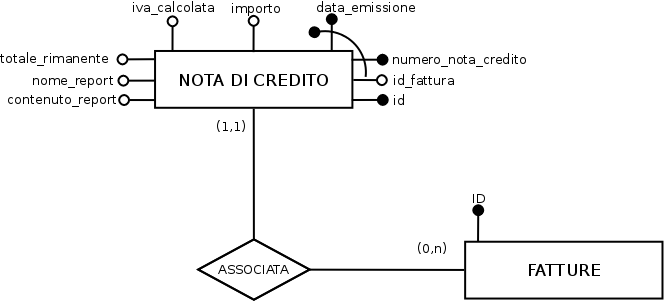
\includegraphics[scale=0.5]{img/schema_concettuale}
\newline
Sono state attuate le seguenti scelte sugli attributi:
\begin{enumerate}
    \item L' attributo \texttt{totale\_rimanente} anche se attributo 
        derivato viene comunque messo per velocizzare le operazioni di 
        visualizzazione delle fatture in modo che non si debba fare ogni volta 
        i calcoli dell’ imponibile con le note di credito.
    \item Sono presenti due chiavi, la prima, chiave primaria, è un \texttt{id} 
        numerico auto incrementante mentre la seconda, chiave canditata, è 
        data dalla coppia \texttt{numero\_nota\_credito} e 
        \texttt{data\_emissione}.
        L'attributo \texttt{id\_fattura} è una chiave esterna ed è associata 
        con l'attributo \texttt{id} che è chiave dell' entità fattura.
    \item Abbiamo due attributi, \texttt{nome\_report} e 
        \texttt{contenuto\_report}, che contegono il nome e il contenuto 
        del file \texttt{.pdf} della nota di credito appena generata.
    \item Sono stati inseriti inoltre solo l’importo e l’ IVA calcolata in 
        quanto la percentuale dell’ IVA utilizzata e l’importo totale della 
        nota di credito possono essere ricavate dagli attributi importo e 
        IVA calcolata.
\end{enumerate}
\subsection{Schema Logico}
Si è quindi passato poi allo schema logico ricavato da quello concettuale.
\newline
\newline
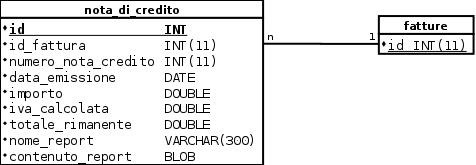
\includegraphics[scale=0.5]{img/schema_logico}
\newline
Come numero di cifre intere è stato scelto undici per rimanere in linea con il
numero di cifre dell' id della tabella \texttt{fattura}
\subsection{Implementazione Fisica}
Il codice della tabella in SQL è il seguente
\lstinputlisting[basicstyle=\ttfamily\scriptsize,title=Codice SQL della tabella]{code/tabella.sql}
Per tutti i campi è stato deciso di renderli tutti non nulli perché alla
generazione della nota di credito tutti i campi devono essere compilati.
\chapter{Implementazione}
Si è passati poi alla scrittura del codice per integrare la nuova funzionalità
nell' applicativo.
Per questa parte sono stato aiutato da due sviluppatori interni all' azienda
di nome Mauro Veronese della sede di Padova e Rocco Spenza della sede di Roma.
\section{Lista delle fatture}
\subsection{Front End}
Per la parte front-end abbiamo deciso come prima cosa di integrare 
l' inserimento delle note di credito all' interno dell' interfaccia 
di inserimento fatture.
\newline
\newline
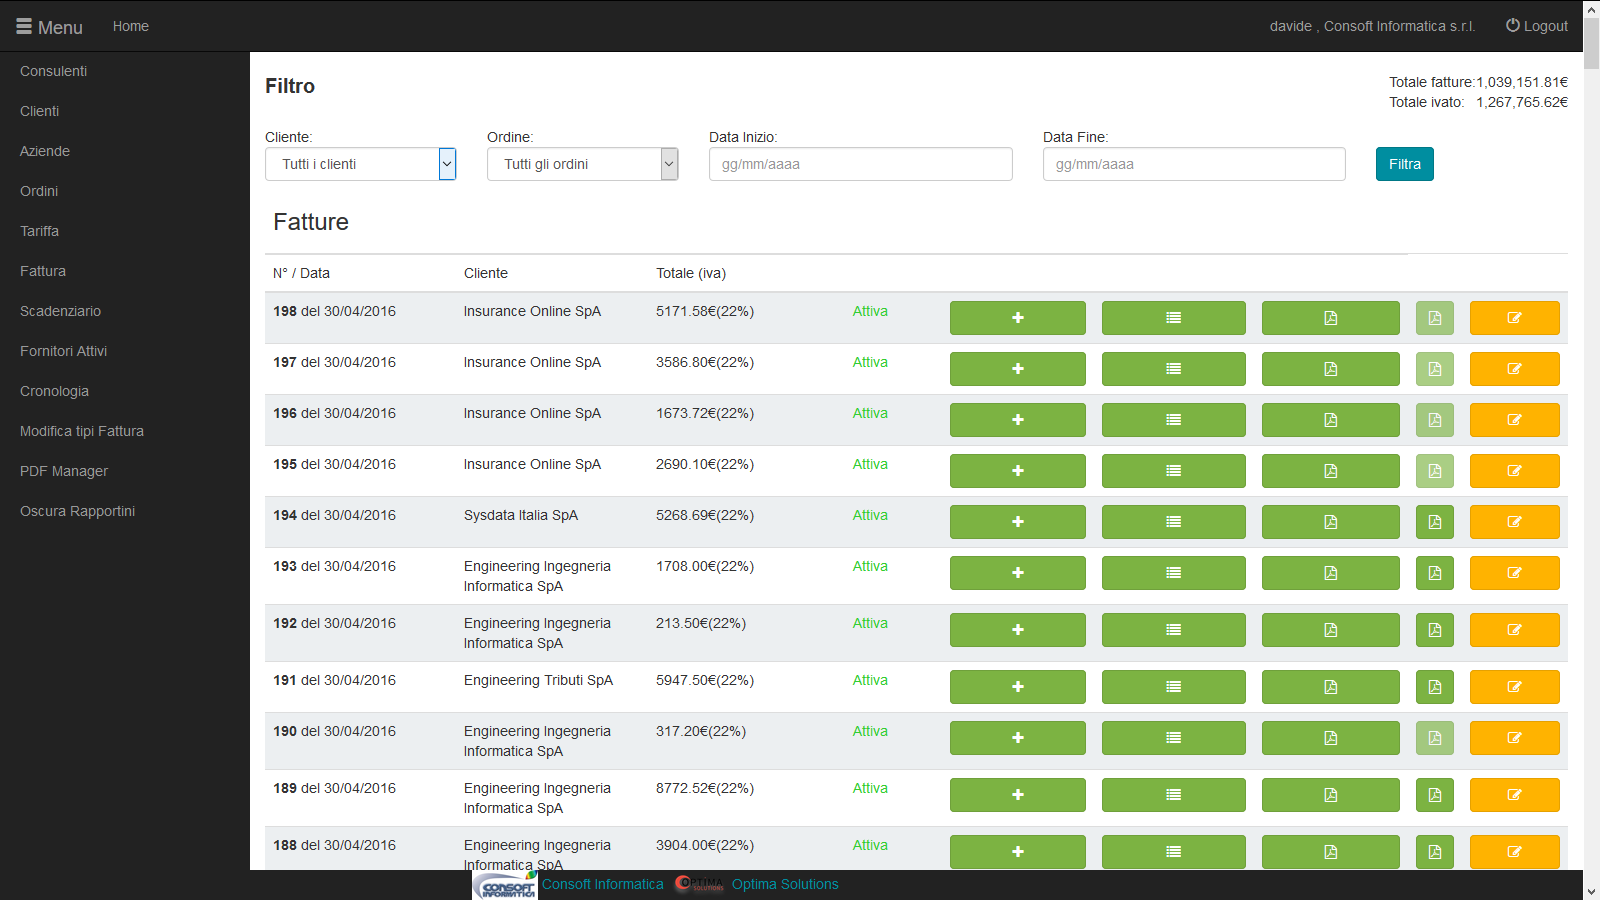
\includegraphics[scale=0.4]{img/lista_fatture}
\newline
I primi due bottoni verdi sono infatti per l' inserimento e la visualizzazione
della nota di credito.
\section{Inserimento della nota di credito}
Dopo aver premuto il tasto 
\begin{thebibliography}{9}
    \bibitem{consoft:descrizione} Sito ufficiale Consoft Informatica \newline
    \texttt{http://www.consoftinformatica.it}
    \bibitem{wikipedia:jsp} Descrizione delle pagine jsp \newline
    \texttt{https://it.wikipedia.org/wiki/JavaServer\_Pages}
\end{thebibliography}
\end{document}



